%%%%%%%%%%%%%%%%%%%%%%%%%%%%%%%%%%%%%%%%%
% Journal Article
% LaTeX Vzor
% Verzia 1.4 (15/5/16)
%
% Tento vzor bol stiahnutý z:
% http://www.LaTeXTemplates.com
%
% Pôvodný autor:
% Frits Wenneker (http://www.howtotex.com) s ďalšími upravami od
% Vel (vel@LaTeXTemplates.com)
%
% Licencia:
% CC BY-NC-SA 3.0 (http://creativecommons.org/licenses/by-nc-sa/3.0/)
%
%%%%%%%%%%%%%%%%%%%%%%%%%%%%%%%%%%%%%%%%%

%----------------------------------------------------------------------------------------
%	PACKAGES A ĎALŠIE UPRAVY DOKUMENTU
%----------------------------------------------------------------------------------------

\documentclass[twoside,twocolumn]{article}

\usepackage{blindtext} % Package to generate dummy text throughout this template 

\usepackage[sc]{mathpazo} % Palatino font
\usepackage[T1]{fontenc} % 8-bitove encodovanie ktore ma 256 glyphov
\linespread{1.10} % Line spacovanie - Palatino potrebuje viacej miesta medzi riadkami
\usepackage{microtype} 

\usepackage[english]{babel}

\usepackage[hmarginratio=1:1,top=32mm,columnsep=20pt]{geometry} % Rozsah dokumentu
\usepackage[hang, small,labelfont=bf,up,textfont=it,up]{caption} % 

\usepackage{booktabs} % Horizontalne pravidla pre tabulky

\usepackage{lettrine} % Prve velke pismeno na zaciatku textu 

\usepackage{enumitem} % Upravitelne listy
\setlist[itemize]{noitemsep} % Make itemize lists more compact

\usepackage{abstract} % Allows abstract customization
\renewcommand{\abstracttextfont}{\normalfont\small\itshape} % Set the abstract itself to small italic text

\usepackage{titlesec} % Allows customization of titles
\renewcommand\thesection{\Roman{section}} % Roman numerals for the sections
\renewcommand\thesubsection{\roman{subsection}} % roman numerals for subsections
\titleformat{\section}[block]{\large\scshape\centering}{\thesection.}{1em}{} % Change the look of the section titles
\titleformat{\subsection}[block]{\large}{\thesubsection.}{1em}{} % Change the look of the section titles

\usepackage{fancyhdr} % Headers and footers
\pagestyle{fancy} % All pages have headers and footers
\fancyhead{} % Blank out the default header
\fancyfoot{} % Blank out the default footer
\fancyhead[C]{Boj proti toxicite a cheatoch v online hrách $\bullet$ Nov 2022} % 
\fancyfoot[RO,LE]{\thepage} % Custom footer text

\usepackage{titling} % Customizing the title section
\usepackage{graphicx}
\usepackage{hyperref} % For hyperlinks in the PDF
\usepackage[export]{adjustbox}

%----------------------------------------------------------------------------------------
%	TITLE SEKCIA
%----------------------------------------------------------------------------------------

\setlength{\droptitle}{-4\baselineskip} % Posun titulku nahor

\pretitle{\begin{center}\Huge\bfseries} % Article titulok formatovanie zaciaotk
\posttitle{\end{center}} % Article titulok formatovanie koniec
\title{Boj proti toxicite a cheatoch v online hrách} % Article titulok
\author{%
\textsc{Jakub Rafaj}\
\\[1ex]
\normalsize Fakulta informatiky a informačných technológií STU v Bratislave  \\%univerzita
\normalsize \href{mailto:rafaj.jakub@gmail.com}{rafaj.jakub@gmail.com} % emailova addresa
}
\date{November 6, 2022} % datum
\renewcommand{\maketitlehookd}{%
}

%----------------------------------------------------------------------------------------

\begin{document}

% Vypisanie titulku
\maketitle

%----------------------------------------------------------------------------------------
%	ARTICLE OBSAH
%----------------------------------------------------------------------------------------
\tableofcontents
\section{Úvod}

\lettrine[nindent=0em,lines=3]{T}oxicita a cheaty\footnote[1]{Externý program, ktorý vám dáva kompetetívnu výhodu.} sú dve veľmi kontroverzné témy, ktoré by sa nemali len tak prehliadať. Preto by som sa v tomto článku chcel pozrieť na ich počiatky, ktoré zapríčinili ich výzor a výskyt v rôznych herných komunitách dnešnej doby. Komunitách populárnych hier ako sú napríklad: League of Legends od spoločnosti RIOT Games alebo Counter Strike Global Offensive od tvorcov VALVE.\\
Taktiež nazrieme na metódy a spôsoby, ako takéto spoločnosti bojujú proti rôznym druhom toxicity prostredníctvom samotných hráčov, ktorí pomocou report systému môžu poukázať na hráča, ktorý takto porušuje pravidlá, ktoré su uvedené v terms of service\footnote[2]{Pravidlá pri prevádzkovaní danej hry.} a ako bojujú proti cheatom\footnotemark[1], ktoré narušujú zábavu a zážitok, takto znevýhodnených hráčov. Ako prostriedky na boj proti cheatom\footnotemark[1] sú určené anti-cheaty\footnote[3]{Program, ktorý zisťuje výskyt cheatov.}, ktorých úlohou je sa zbavovať hráčov, ktorí takéto externe third party programy\footnote[4]{Program, ktorý pracuje mimo danej hry.} používajú vo svoj prospech, aby si vylepšili svoj herný výsledok, výkon a počet vyhraných hier, ktorý sa potom vykresľuje na ich výslednom ranku\footnote[5]{Ohodnotenie hráča podľa jeho herného výkonu.}.

%------------------------------------------------

\section{Metódy}

V tejto sekcii sú uvedené metódy boja proti toxicite a cheatom\footnotemark[1].
\begin{itemize}
\item Terms of service\footnotemark[2] 
\item Report systém\footnote[6]{Nahlásovanie hráčov hráčmi.}
\item Anti-cheat\footnotemark[3]
\item Bannovanie\footnote[7]{Zákaz spustenia kompetetívnej hry na určitú dobu.}
\item Chat\footnote[8]{Prostredie na písanie pre hráčov.} reštrikcia
\end{itemize}
	Po inštalácii hry, hráči musia potvrdiť terms of service\footnotemark[2]t.j. kliknutí na tlačítko "Accept",čo značí potvrdenie. Terms of service\footnotemark[2] majú informovať hráča o rôznych priestupkoch, ktorých sa hráči nesmú dopustiť, ak nechcú byť potrestaný. Ak sa hráč dopustil priestupku a je zaznamenaný systémom, najčastejšie prostredníctvom anti-cheatu\footnotemark[3], alebo nahlásením tohto hráča iným hráčom.\\
	Report systém\footnote[1]{Nahlasovanie hráčov hráčmi.} je jeden zo spôsobov, zachytávania priestupkov, ktorých sa hráči bežne dopúšťajú. Tieto priestupky sú následne ohlásené do systému hráčom, ktorý je vedomý priestupku, ktorého sa druhý hráč dopustil, alebo práve dopúšťa. Následne sú tieto sťažnosti od hráčov preverené ľuďmi na to určenými. Títo ľudia overia pravdivosť sťažností a korektne potrestajú daného hráča, ktorý sa dopustil priestupku.\\
	Anti-cheat\footnote[2]{Program, ktorý zisťuje výskyt cheatov.} je program, ktorý je naprogramovaný na to, aby kontroloval hráčov a následne zistil výskyt third party programu\footnote[3]{Program, ktorý pracuje mimo danej hry.}, ktorý hráč používa, ako kompetetívnu výhodu a následne je korektne potrestaný.\\
	Banovanie\footnote[4]{Zákaz spustenia kompetetívnej hry na určitú dobu.} je spôsob trestania hráčov, ktorí sa dopustili priestupku, ktorý je v rozpore s terms of service\footnote[5]{Pravidlá pri prevádzkovaní danej hry.}. Ak je hráč zabanovaný\footnotemark[4], tak je mu na určitý čas odoprená možnosť pripojiť sa do kompetetívnej hry. Ak samotný hráč neustále porušuje terms of service\footnotemark[5], tak jednotlivé bany časovo trvajú dlhšie a dlhšie, až do momentu, kedy sú permanentné\footnote[6]{Navždy.}.   \\
	Chat\footnote[7]{Prostredie na písanie pre hráčov.} restrikcia je spôsob, akým hry zakazujú hráčom, ktorí porušili terms of service\footnotemark[5],na určitý čas písanie do chatu.

%------------------------------------------------

\section{Anti-cheat}
\subsection{Machine learning}
Machine Learning je jeden z typov anti-cheatov\footnotemark[3], ako je písané v \cite{willman2020machine}. Tento anti-cheat\footnotemark[3] pracuje a vyhodnocuje svoje rozhodnutia na základe algoritmu\footnote[8]{Spôsob, podľa ktorého program vyhodnocuje svoje rozhodnutia.}, ktorý bol naprogramovaný človekom a na základe toho, či bolo to rozhodnutie správne , alebo chybné je algoritmus\footnotemark[8] zmenený a vylepšený človekom. Čím viacej informácii program dostáva v algoritme\footnotemark[8], tým je výsledok presnejší. Tento proces učenia je klasifikovaný ako rýchly. \\
Machine learning funguje na podnetoch/vstupoch, ktoré získava z danej hry, následne tieto podnety/vstupy vyhodnocuje pomocou algoritmu\footnotemark[8] a po vyhodnocovaní vykoná akciu/výstup, ktorý je buď správny, alebo nesprávny.\\

\textnormal{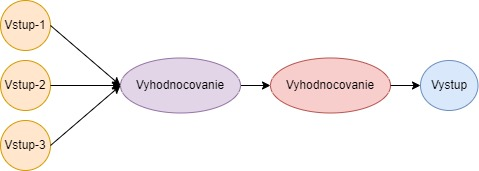
\includegraphics[scale=0.42]{Machine learning proces diagram.jpg}}
\label{machine learning proces}


\subsection{Deep Learning}
Deep Learning je funguje na rovnaký systém, ako Machine learning, lenže tento systém na rozdiel od machine learningu nepotrebuje človeka na vylepšovanie, ale vylepšuje sa sám a to pomocou svojich skúseností a rozhodnutí, ako je aj písané v \cite{zhang2021improvement}. Nevýhodou systému na základe deep learningu je, že proces učenia trvá značne dlhšie, ako pri machine learningu, ktorý je programovaný človekom, ale ak uplynie dostatok času rozhodnutia tohto systému sú priemerom presnejšie ako pri machine learningu.
Deep learning je vylepšenie machine learningu, pričom deep learning pracuje pomocou techniky machine learningu, ktorá rozdeľuje algoritmy\footnotemark[8] a neuróny do takzvanej umelej neurónovej site. Neurónová sieť je vytvorená, tak aby pracovala a operovala na rovnaký spôsob ako náš ľudský mozog.
\newpage

%------------------------------------------------

\section{Toxicita}

	Toxicita v hrách sa vyskytuje na dennej báze. Ak už ste niekedy hrali online hru, tak určite ste zažili, konflikt v chate\footnote{Prostredie na písanie pre hráčov.}, alebo voice-chate\footnote{Prostredie na ústnu komunikáciu pre hráčov.} medzi dvoma, alebo aj viac hráčmi, či už tí hráči boli z vášho tímu, alebo to bol konflikt medzi vašim tímom a nepriteľským tímom. Tieto konflikty sú z väčšej časti vyprodukované hráčmi, ktorí sú v zápale hry a v ten moment tímto hráčom sú terms of service\footnote{Pravidlá pri prevádzkovaní danej hry.}a následky, za ktoré neskôr budú musieť zodopovedať, ukradnuté. Aj ja osobne, ako hráč online hier sa bežne stretávam s toxicitou. Táto toxicita je prevažne jemná, ale občas sa stane, že toxicita začne presahovať všetky medze.V takomto prípade nahlasujem hráčov pomocou report systému\footnote{Nahlasovanie hráčov hráčmi.}.\\
	V dnešnej dobe avšak jednotlivé spoločnosti z časti tolerujú jemnú toxicitu, pretože nie každý konflikt medzi hráčmi je hneď vyprovokovaný nenávisťou, ale je to skôr, škádlenie a pošťuchovanie súpera. Nejeden hráč si zapne hru práve kvôli tomu, aby si mohol zo súpera robiť srandu.\\
	Problém nastáva, keď táto toxicita vyvrcholí do takého bodu, kedy už nemá hranice a hráči si napríklad navzájom prajú smrť, alebo ďalšie hrozné veci. Takúto štatistickú analýzu môžete nájsť aj v článku \cite{ghosh2021analyzing}, kde sú zachytené slova a typy slov, ktoré sú na toxicitu medzi hráčmi bežne používané.\\ 
	Proti hrubej toxicite jediné, čo môžu herné spoločnosti spraviť, je ju nejakým určitými spôsobmi obmedziť. A nato slúži práve chat\footnote{Prostredie na písanie pre hráčov.} reštrikcia, alebo ak chat reštrikcia nepomáha a daný hráč neustále zachádza príliš ďaleko, tak aj bany\footnote{Zákaz spustenia kompetetívnej hry na určitú dobu.} sú použité na potrestanie tohto hráča.\\
\newpage

%----------------------------------------------------------------------------------------
%	REFERENCE LIST
%----------------------------------------------------------------------------------------

% Bibliografia
\bibliographystyle{elsarticle-num}
\bibliography{bibliography}

%----------------------------------------------------------------------------------------

\end{document}
